\chapter{Appendix - Chapter 3}
\label{ch:appendix_ch3}

\section{Figures}

\begin{figure}[H]
    \centering
    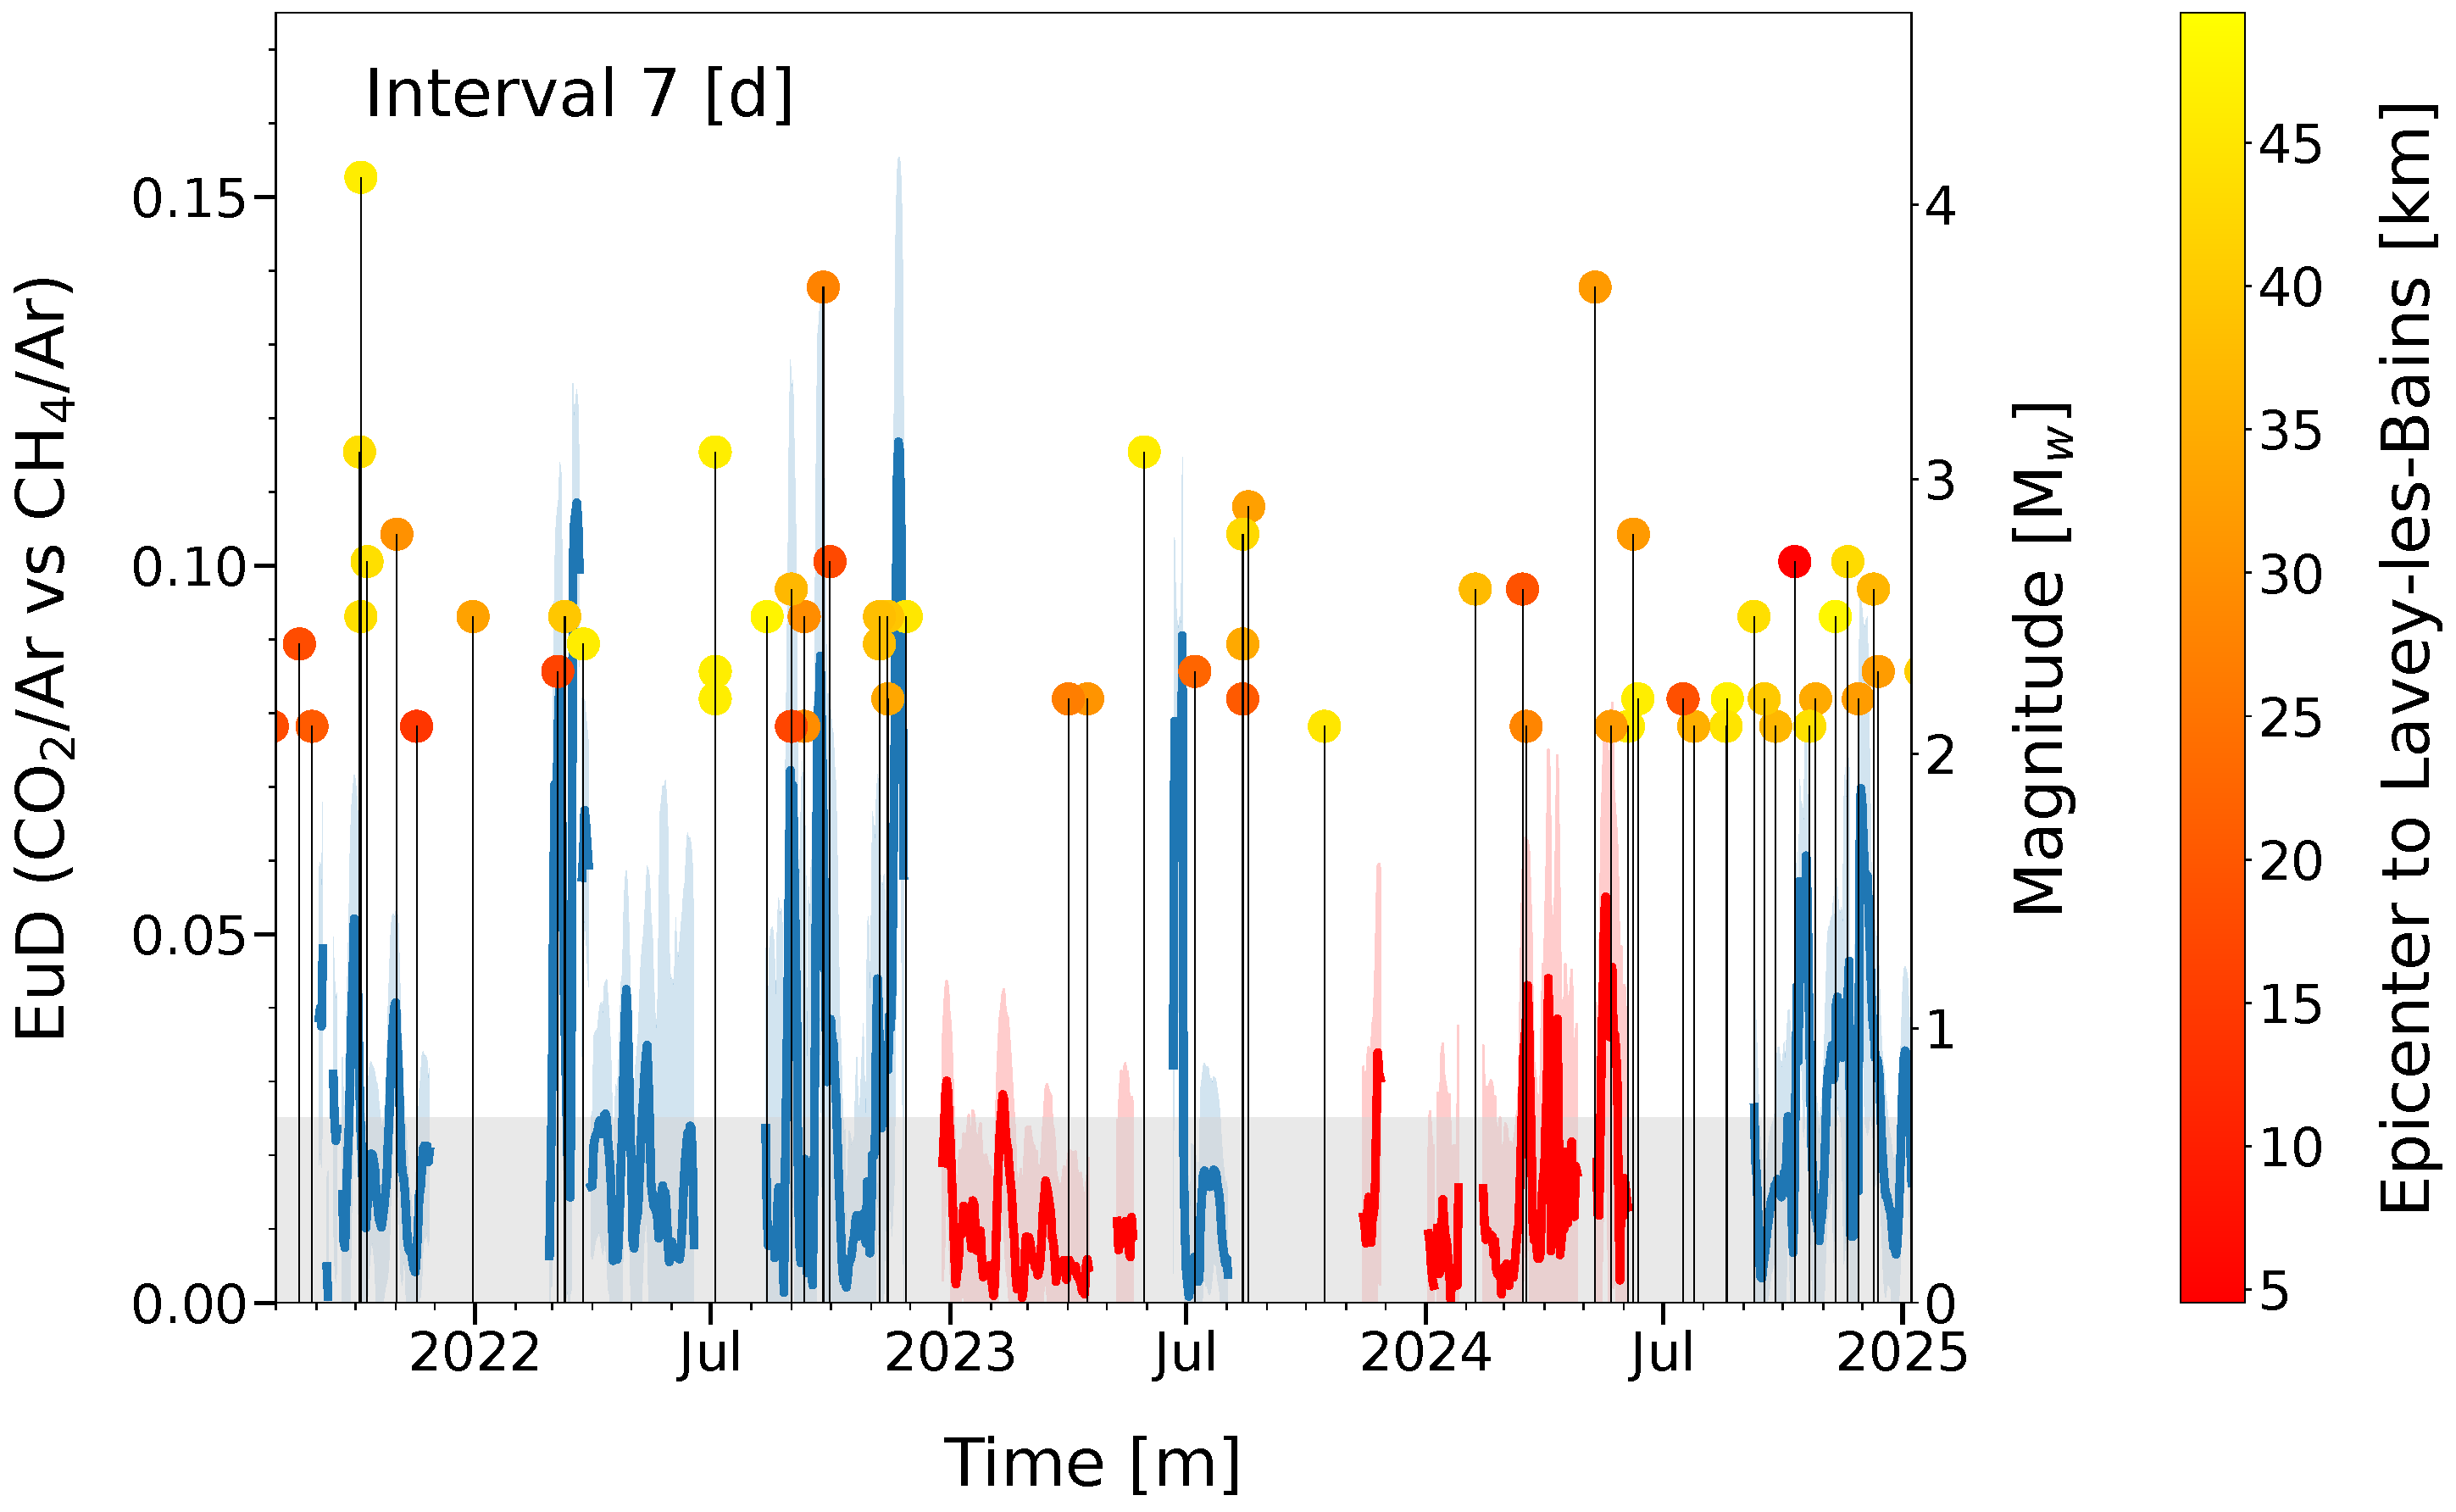
\includegraphics[width=0.75\textwidth]{chapters/06_appendix/SI_C3/full_EuD_7.pdf}
    \caption{
    EuD values for \ce{CO2}/Ar versus \ce{CH4}/Ar in wells P201 (blue) and P600 (red), computed using a 7-day interval from September 2021 to January 2025.
    Shaded areas indicate propagated uncertainties.
    The secondary y-axis displays earthquake magnitudes (M$_w \geq 2.0$) within \SI{50}{\kilo\meter} of Lavey-les-Bains; point color denotes epicentral distance (warmer hues = closer proximity).
    The gray band represents a fixed noise threshold of 0.025, used due to variable baseline uncertainty.
    }
    \label{figSI:full_EuD_EuD7}
\end{figure}

\begin{figure}[H]
    \centering
    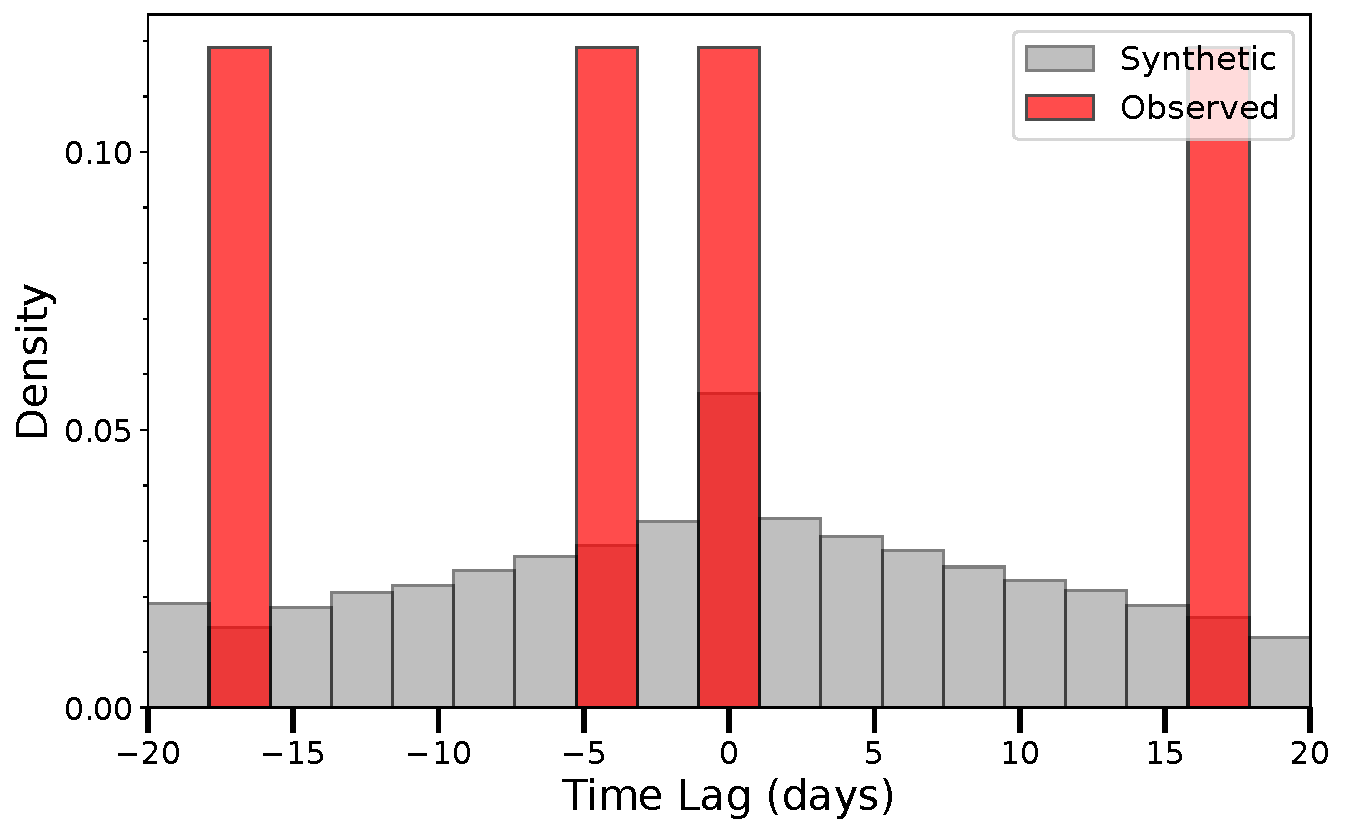
\includegraphics[width=0.75\textwidth]{chapters/06_appendix/SI_C3/distribution_earthquakes_wo_outliers_well_600.pdf}
    \caption{
    Distribution of time lag between EuD maxima in well P600 and regional earthquakes (red, observed data; M$_w \geq 2.0$, within \SI{50}{\kilo\meter} of Lavey-les-Bains), compared to a synthetic distribution of randomly generated earthquakes (grey, synthetic data; \num{10000} iterations).
    A maximum time lag threshold of \SI{18}{\day} was applied to both distributions.
    Negative values indicate that EuD maxima occurred before the corresponding earthquake, and positive values indicate they occurred after.
    Both distributions are centered on zero.
    }
    \label{figSI:distributions_P600}
\end{figure}